\documentclass{beamer}

\usepackage{beamerthemesplit}

\title{Zero to Root in 12 Months}
\subtitle{Training and Utilizting Junior Sysadmins in Higher Education}
\date{\today}
\author{Spencer Krum, William Van Hevelengin}

\begin{document}

\frame{\titlepage}

% Slide 
\section{Introduction}
\subsection{Presenters}
\frame 
{
    \frametitle{Presenters}
        \begin{columns}[c]
        \column{.5\textwidth}
        \begin{center}
        Spencer Krum\\
        nibz@cat.pdx.edu\\
        \end{center}
        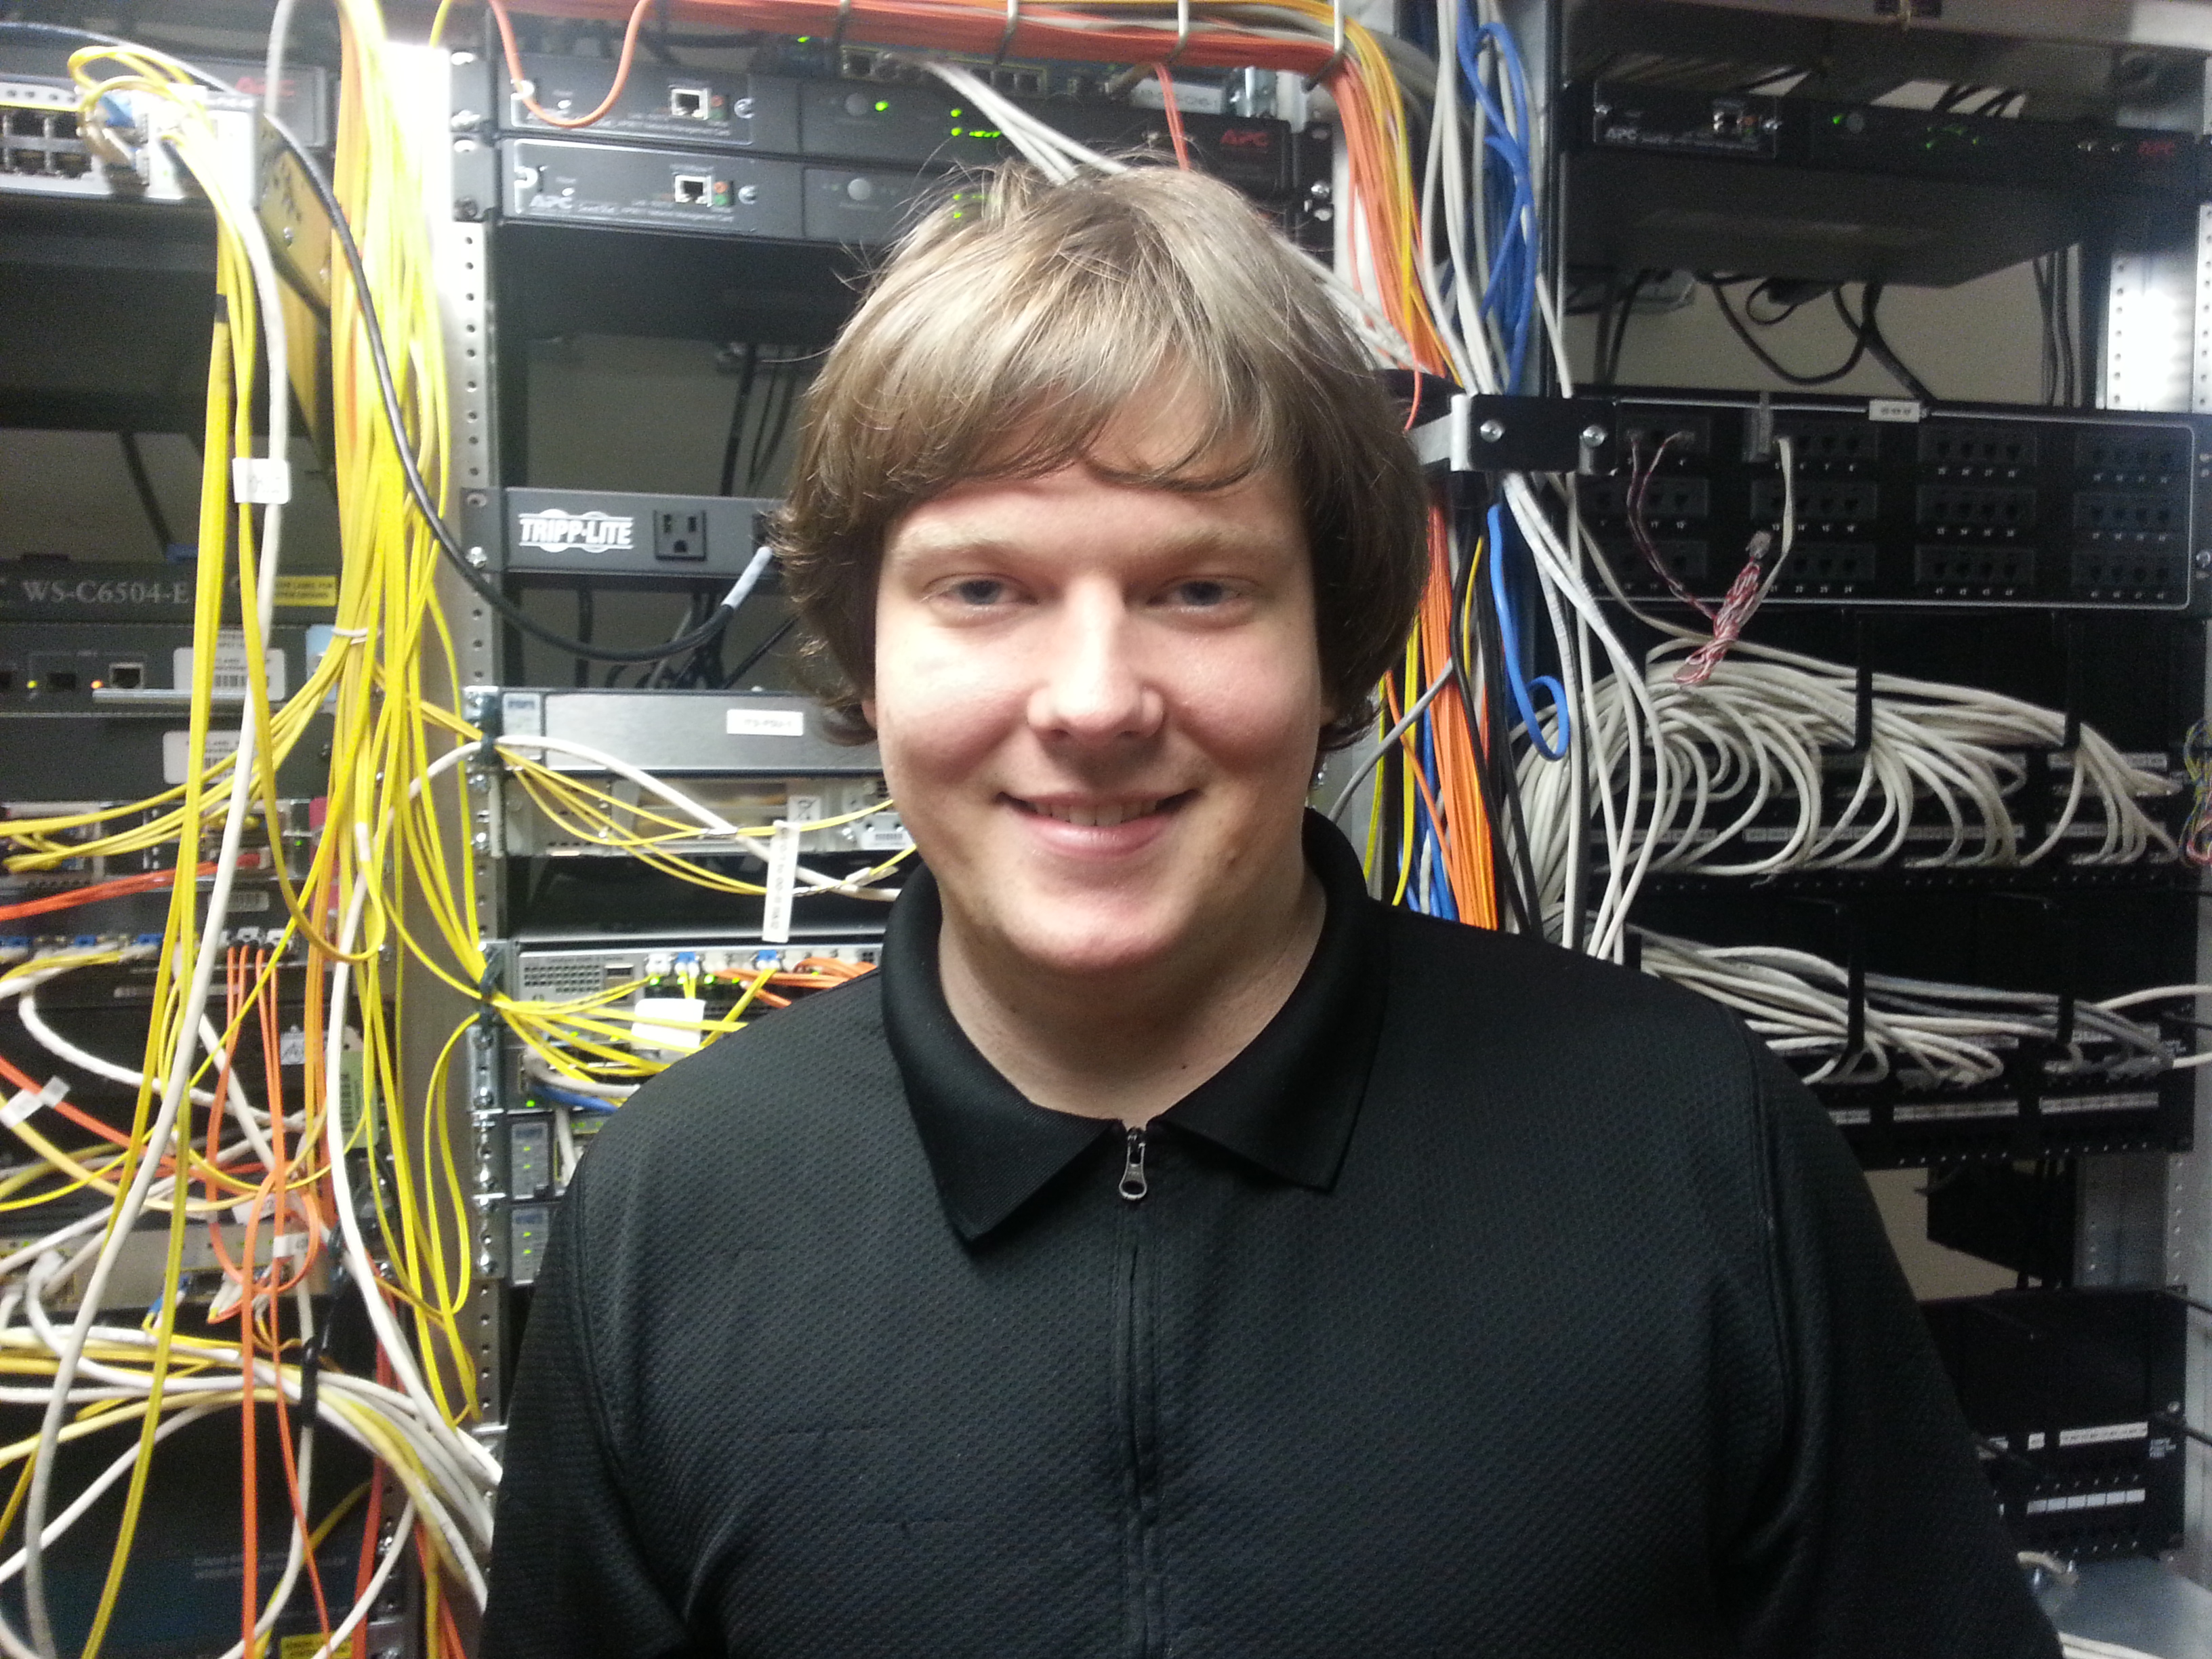
\includegraphics[width=1\textwidth]{spencer.jpg}
        
        \column{.5\textwidth}
        \begin{center}
        William Van Hevelengin\\
        blkperl@cat.pdx.edu\\
        \end{center}
        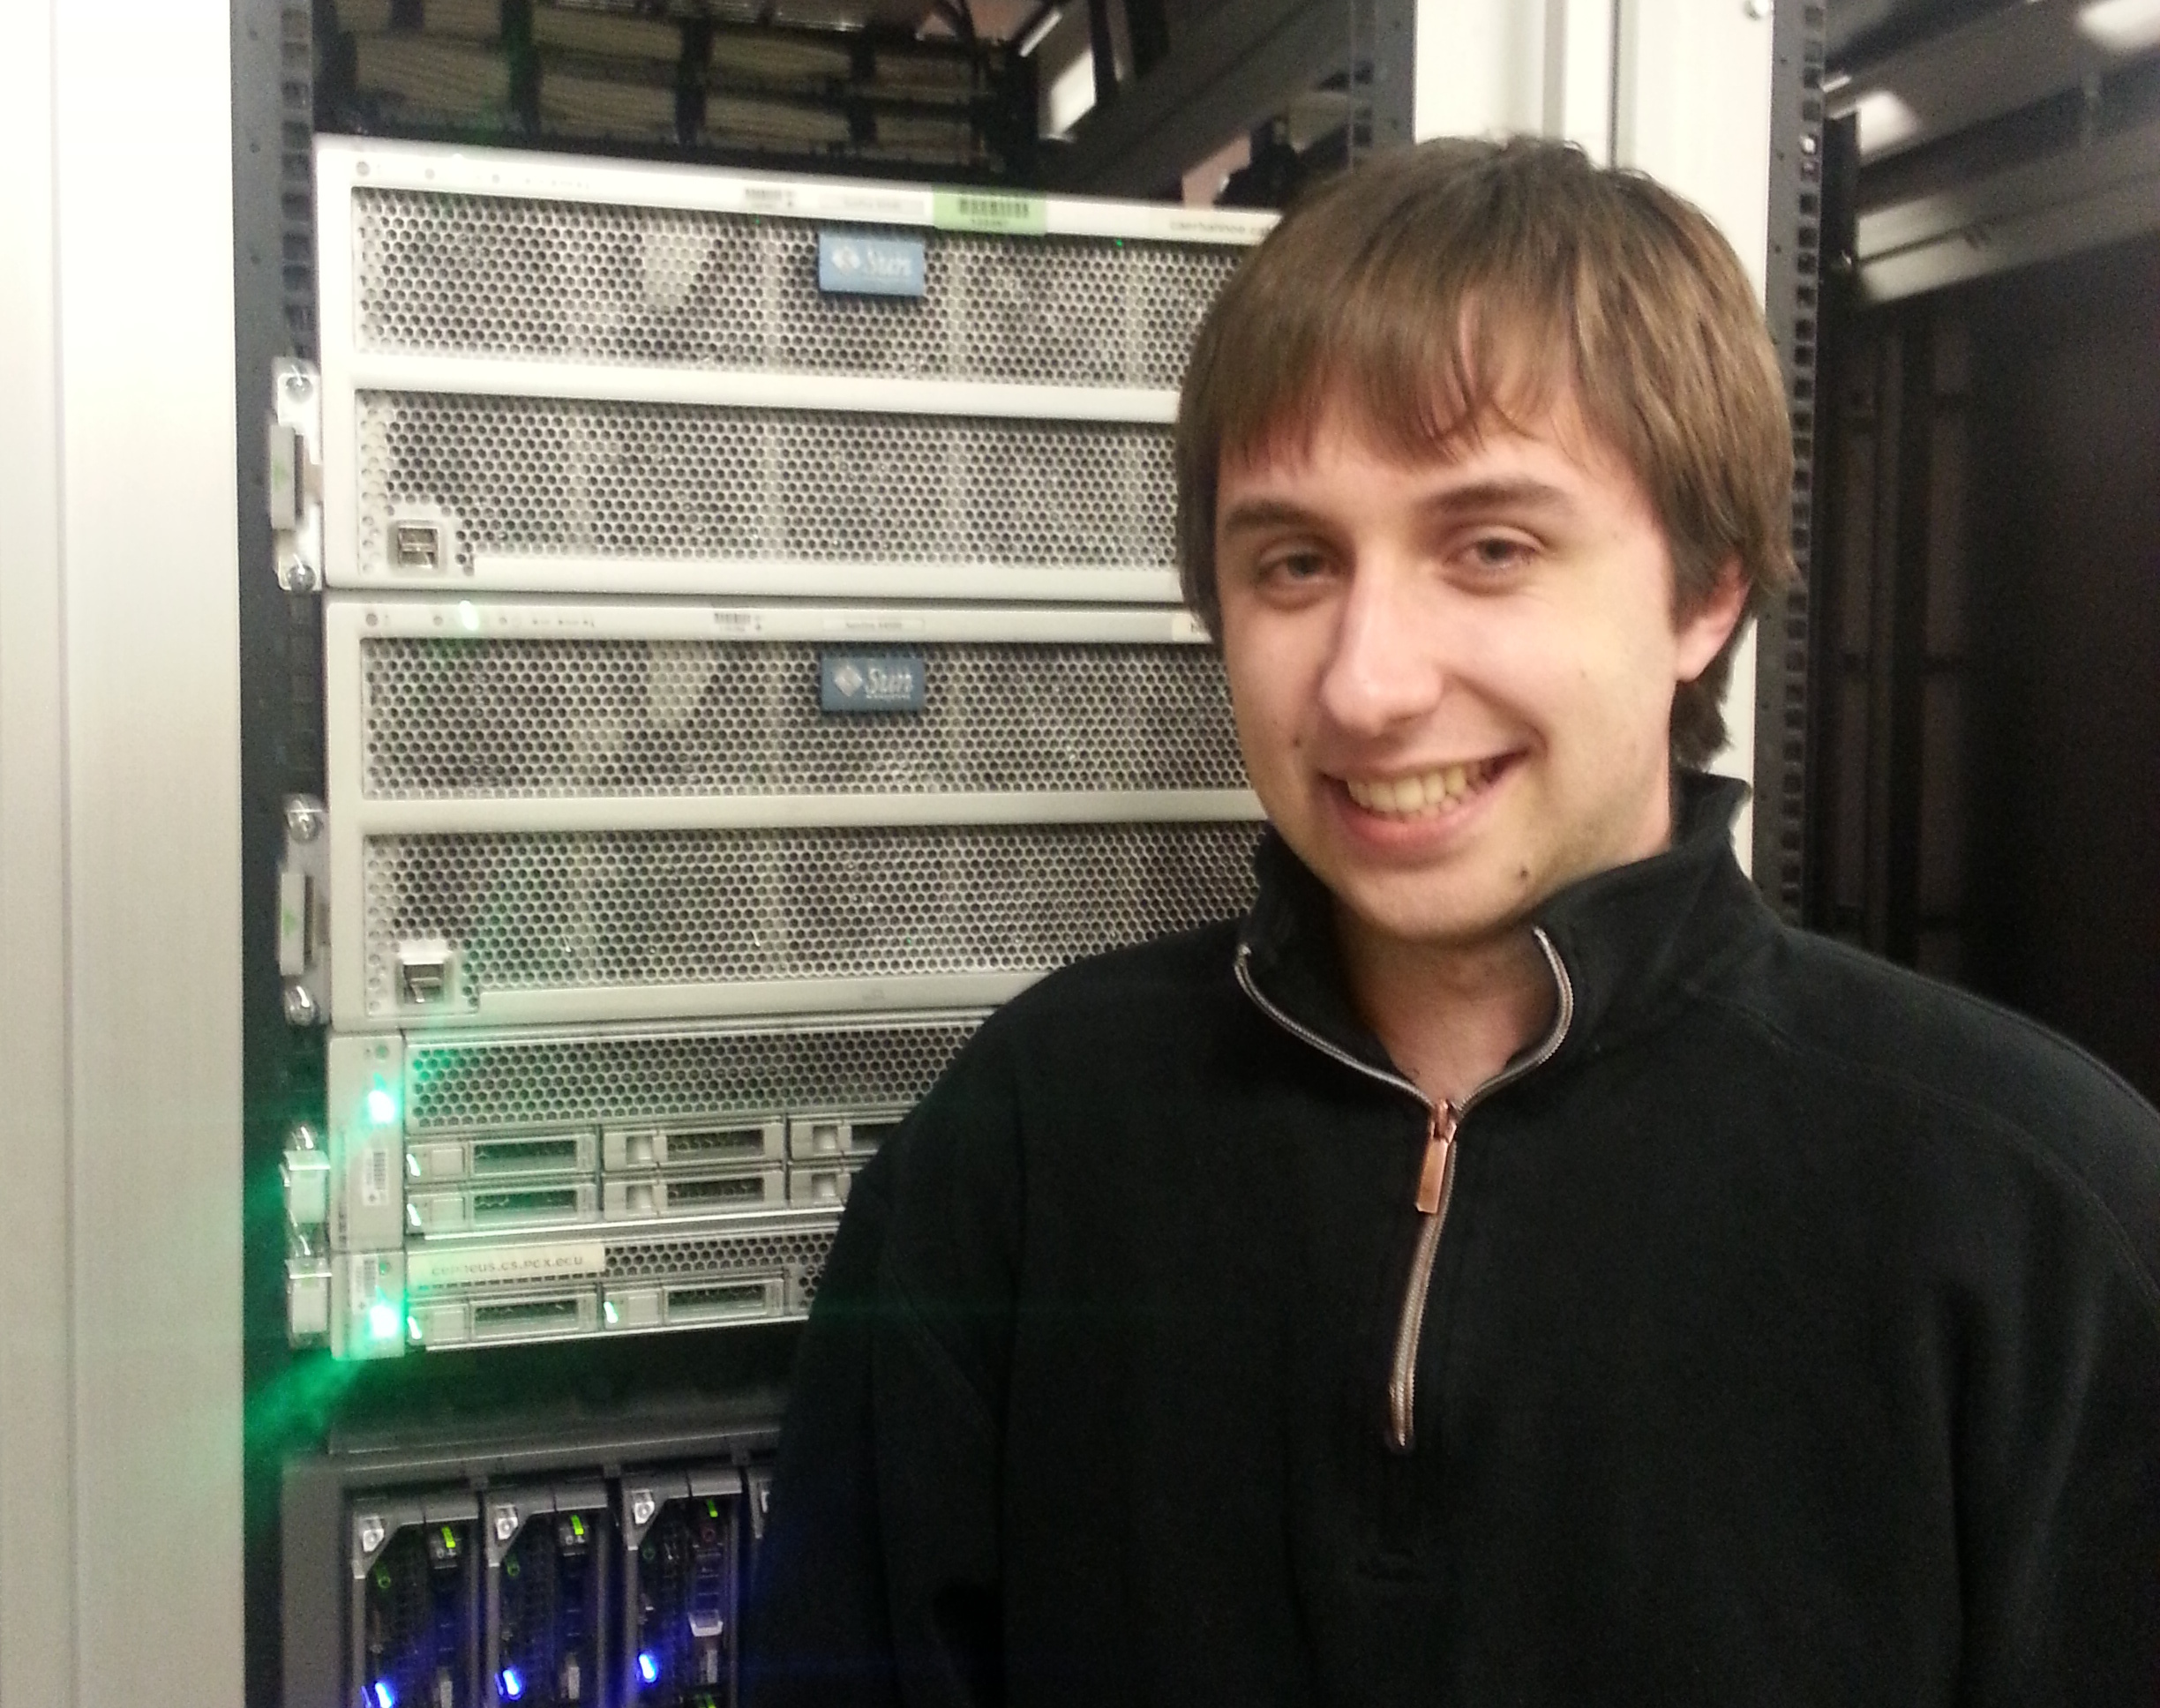
\includegraphics[width=1\textwidth]{blkperl.jpg}
        \end{columns}
}
% Slide 
\subsection{Agenda}
\frame
{
    \frametitle{Agenda}
    \begin{itemize}
        \item Computer Action Team introduction and history
        \item Braindump progradm
        \item Utilization
        \item Personal Stories
    \end{itemize}
}

% Slide
\section{Computer Action Team}
\subsection{Stats}
\frame
{
    \frametitle{Stats}
    \begin{itemize}
        \item 4 Buildings
        \item 5K users
        \item 600 Workstations, 100 Server
        \item 7 general use computer labs
        \item Manage hundreds of commercial and OSS software pkgs
        \item 1854 active networking jacks
        \item 2x10 Gigabit Ethernet links to the internet
    \end{itemize}

}

\subsection{Operating Systems}
\frame
{
    \frametitle{Operating Systems}
    \begin{itemize}
        \item Windows
        \item Ubuntu
        \item RedHat/Centos
        \item Solaris/Derviatives
    \end{itemize}
}

% Slide
\subsection{CAT Services}
\frame
{
    \frametitle{CAT Services}
    \begin{itemize}
        \item Web
        \item License management
        \item Network homedirs
        \item Bulk storage over NFS/Samba
        \item Database (mysql/postgres)
        \item Project Management & VCS
        \item Backups
        \item VPN
        \item Networking
        \item Mail
    \end{itemize}

}

% Slide
\section{Braindump}
\subsection{Background}
\frame
{
    \frametitle{Background}
    \begin{itemize}
        \item Founded in early 90s by Janaka Jayawardena, Director of IT for Engineering
        \item Originally a means by Janaka to grow UNIX hackers that got out of hand.
        \item In-house apprenticeship program to bring student volunteers into sysadmin and other IT roles.
        \item Hire them later (once they know what they are doing)
    \end{itemize}
}

% Slide
\subsection{Particulars}
\frame
{
    \frametitle{Particulars}
    \begin{itemize}
        \item 1+ yr program
        \item Open to any PSU student/staff
        \item Friday nights, 6pm-10pm
        \item 4 hours helpdesk volunteering a week
        \item Time, as needed, spent working on learning and projects.
    \end{itemize}
}

% Slide
\subsection{Challenges}
\frame
{
    \frametitle{Things that have tripped us up}
    \begin{itemize}
        \item Noise
        \item Sensor drift
        \item The accelerometer conspiracy
        \item The super-tool problem
        \item The leaf problem
        \item Cosine function
    \end{itemize}
}
% Slide
\subsection{Milestones}
\frame
{
    \frametitle{Really cool things that happened}
    \begin{itemize}
        \item Greg wrote an RTOS
        \item Bribed mechanical engineers
        \item Kept the number of `black boxes' to an absolute minimum
        \item Set up foodbot
    \end{itemize}
}

% Slide
\section{Budget}
\subsection{Overview}
\frame
{
\footnotesize{    
\begin{center}
\begin{tabular}[t]{lr}
 Flight Components:   &\\
\indent \it  Carbon Fiber Frame                    &\$100.00\\
\indent \it  2 Motors                               &\$89.98\\
\indent \it  PCB ESCs                              &\$100.00\\
\indent \it  Battery Charger                       &\$119.99\\
\it                                        &\textbf{\$410.97}\\
 Navigation Components: &\\
\indent \it  PandaBoard Minicomputer               &\$174.00\\
\indent \it  Printed PCB and components (control)  &\$200.00\\
\indent \it  Printed PCB and components (power)    &\$100.00\\
\indent \it  Digital inertial measurement unit      &\$64.95\\
\indent \it  Protoboard and components             &\$100.00\\
\it                                        &\textbf{\$638.95}\\
 Miscellaneous:                       &\\
\indent \it  Testing Equipment                     &\$100.00\\
\indent \it  Unplanned Expenditures(S\&H)          &\$200.00\\
\it                                        &\textbf{\$300.00}\\\hline
 Total:                                   &\textbf{\$1316.84}\\
\end{tabular}
\end{center}
}
}

% Slide
\section{Outro}
\subsection{Thank You}
\frame
{
    \frametitle{Thank You very much}

    \begin{itemize}
        \item Once again, we're the PSU Remote Operated Vehicle Team
        \item I, and my teammates as well, strongly support this pilot program because our experience last year with getting involved in student engineering was the highlight of my college experience to date. 
        \item Thanks Again!
    \end{itemize}
}

% Slide
\subsection{Want to Join?}
\frame
{
    \frametitle{We want you}

    \begin{itemize}
        \item Google Group - psu-rov@googlegroups.com
        \item Redmine - rov.cs.pdx.edu
        \item Weekly Meetings - FABc 86-04 - 1:00pm Saturdays
        \item IRC \#rov, irc.cat.pdx.edu
    \end{itemize}
}
\end{document}

